\begin{frame}{Stateful Firewall}
    \begin{center}
        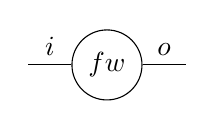
\begin{tikzpicture}[node distance={15mm},main/.style = {draw, circle}]
            \node[main] (s) {$fw$};
            \draw (s) -- node[above]{$i$} (-1,0);
            \draw (s) -- node[above]{$o$} (1,0);
        \end{tikzpicture}
    \end{center}
    Correct Behavior:
    \begin{itemize}
        \item Allow outgoing packets
        \item Drop incoming packets
        \item Allow incoming packets once a packet sent outside
    \end{itemize}
\end{frame}

\begin{frame}
    \begin{center}
        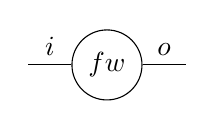
\begin{tikzpicture}[node distance={15mm},main/.style = {draw, circle}]
            \node[main] (s) {$fw$};
            \draw (s) -- node[above]{$i$} (-1,0);
            \draw (s) -- node[above]{$o$} (1,0);
        \end{tikzpicture}
        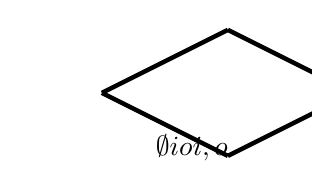
\begin{tikzpicture}[scale=0.8]
            \crd{0}{0}{$\emptyset$}
            \crd[left]{-2}{1}{$\s{i}$}
            \crd[right]{2}{1}{$\s{o}$}
            \crd[right]{0}{2}{$\s{i,o}$}
            \draw [ultra thick] (0,0) -- (2,1);
            \draw [ultra thick] (0,0) -- (-2,1);
            \draw [ultra thick] (-2,1) -- (0,2);
            \draw [ultra thick] (2,1) -- (0,2);
        \end{tikzpicture}
    \end{center}
    \begin{itemize}
        \item Counterexample: $\sigma = \s{o}$
        \item Cause: $M(\s{i},o) = \F$
        \item Conditions:
    \end{itemize}
    \begin{align*}
        \m & \vDash M(\s{i},o) = \F \wedge \sigma \in
        \mathcal{F}(\mathrm{E})                        \\
        \m & \vDash [M(\s{i},o)\la \T] \sigma \not \in
        \mathcal{F}(\mathfrak{E}(\vec V)) \wedge \vec V = \vec v
        \wedge \vec v \in \mathcal{E}
    \end{align*}
\end{frame}

\begin{frame}
    \begin{center}
        \begin{tikzpicture}[node distance=15mm]
            \node[r] (moi) {$M_{\s{o},i}$};
            \node[b] (mei) [below right of=moi] {$M_{\e,i}$};
            \node[b] (eei) [below of=mei] {$EN_{\e,i}$};
            \node[b] (eoi) [below left of=eei]{$EN_{\s{o},i}$};
            \draw[->] (moi) -- (mei);
            \draw[->] (mei) -- (eei);
            \draw[->] (eei) -- (eoi);
            \draw[->] (moi) -- (eoi);

            \node[r] (mio) [left of=moi] {$M_{\s{i},o}$};
            \node[b] (meo) [below left of=mio] {$M_{\e,o}$};
            \node[b] (eeo) [below of=meo] {$EN_{\e,o}$};
            \node[b] (eio) [below right of=eeo]{$EN_{\s{i},o}$};
            \draw[->] (mio) -- (meo);
            \draw[->] (meo) -- (eeo);
            \draw[->] (eeo) -- (eio);
            \draw[->] (mio) -- (eio);
        \end{tikzpicture}
        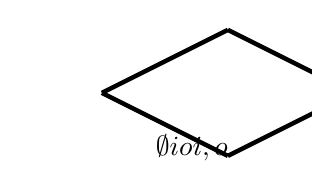
\begin{tikzpicture}[scale=0.8]
            \crd{0}{0}{$\emptyset$}
            \crd[left]{-2}{1}{$\s{i}$}
            \crd[right]{2}{1}{$\s{o}$}
            \crd[right]{0}{2}{$\s{i,o}$}
            \draw [ultra thick] (0,0) -- (2,1);
            \draw [ultra thick] (0,0) -- (-2,1);
            \draw [ultra thick] (-2,1) -- (0,2);
            \draw [ultra thick] (2,1) -- (0,2);
        \end{tikzpicture}
    \end{center}
\end{frame}
\begin{frame}
    \begin{center}
        \begin{tikzpicture}[node distance=15mm]
            \node[r] (moi) {$M_{\s{o},i}$};
            \node[b] (mei) [below right of=moi] {$M_{\e,i}$};
            \node[b] (eei) [below of=mei] {$EN_{\e,i}$};
            \node[b] (eoi) [below left of=eei]{$EN_{\s{o},i}$};
            \draw[->] (moi) -- (mei);
            \draw[->] (mei) -- (eei);
            \draw[->] (eei) -- (eoi);
            \draw[->] (moi) -- (eoi);

            \node[o] (mio) [left of=moi] {$M_{\s{i},o}$};
            \node[b] (meo) [below left of=mio] {$M_{\e,o}$};
            \node[b] (eeo) [below of=meo] {$EN_{\e,o}$};
            \node[b] (eio) [below right of=eeo]{$EN_{\s{i},o}$};
            \draw[->] (mio) -- (meo);
            \draw[->] (meo) -- (eeo);
            \draw[->] (eeo) -- (eio);
            \draw[->] (mio) -- (eio);
        \end{tikzpicture}
        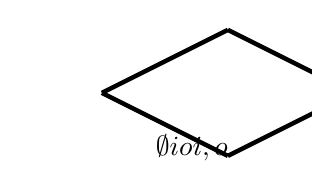
\begin{tikzpicture}[scale=0.8]
            \crd{0}{0}{$\emptyset$}
            \crd[left]{-2}{1}{$\s{i}$}
            \crd[right]{2}{1}{$\s{o}$}
            \crd[right]{0}{2}{$\s{i,o}$}
            \draw [ultra thick] (0,0) -- (2,1);
            \draw [ultra thick] (0,0) -- (-2,1);
            \draw [ultra thick] (-2,1) -- (0,2);
            \draw [ultra thick] (2,1) -- (0,2);
        \end{tikzpicture}
    \end{center}
\end{frame}

\begin{frame}
    \begin{center}
        \begin{tikzpicture}[node distance=15mm]
            \node[r] (moi) {$M_{\s{o},i}$};
            \node[b] (mei) [below right of=moi] {$M_{\e,i}$};
            \node[b] (eei) [below of=mei] {$EN_{\e,i}$};
            \node[b] (eoi) [below left of=eei]{$EN_{\s{o},i}$};
            \draw[->] (moi) -- (mei);
            \draw[->] (mei) -- (eei);
            \draw[->] (eei) -- (eoi);
            \draw[->] (moi) -- (eoi);

            \node[b] (mio) [left of=moi] {$M_{\s{i},o}$};
            \node[o] (meo) [below left of=mio] {$M_{\e,o}$};
            \node[b] (eeo) [below of=meo] {$EN_{\e,o}$};
            \node[o] (eio) [below right of=eeo]{$EN_{\s{i},o}$};
            \draw[->] (mio) -- (meo);
            \draw[->] (meo) -- (eeo);
            \draw[->] (eeo) -- (eio);
            \draw[->] (mio) -- (eio);
        \end{tikzpicture}
        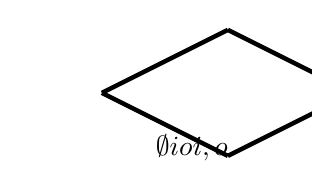
\begin{tikzpicture}[scale=0.8]
            \crd{0}{0}{$\emptyset$}
            \crd[left]{-2}{1}{$\s{i}$}
            \crd[right]{2}{1}{$\s{o}$}
            \crd[right]{0}{2}{$\s{i,o}$}
            \draw [ultra thick] (0,0) -- (2,1);
            \draw [ultra thick] (0,0) -- (-2,1);
            \draw [ultra thick] (-2,1) -- (0,2);
            \draw [ultra thick] (2,1) -- (0,2);
        \end{tikzpicture}
    \end{center}
\end{frame}

\begin{frame}
    \begin{center}
        \begin{tikzpicture}[node distance=15mm]
            \node[r] (moi) {$M_{\s{o},i}$};
            \node[b] (mei) [below right of=moi] {$M_{\e,i}$};
            \node[b] (eei) [below of=mei] {$EN_{\e,i}$};
            \node[b] (eoi) [below left of=eei]{$EN_{\s{o},i}$};
            \draw[->] (moi) -- (mei);
            \draw[->] (mei) -- (eei);
            \draw[->] (eei) -- (eoi);
            \draw[->] (moi) -- (eoi);

            \node[b] (mio) [left of=moi] {$M_{\s{i},o}$};
            \node[r] (meo) [below left of=mio] {$M_{\e,o}$};
            \node[o] (eeo) [below of=meo] {$EN_{\e,o}$};
            \node[b] (eio) [below right of=eeo]{$EN_{\s{i},o}$};
            \draw[->] (mio) -- (meo);
            \draw[->] (meo) -- (eeo);
            \draw[->] (eeo) -- (eio);
            \draw[->] (mio) -- (eio);
        \end{tikzpicture}
        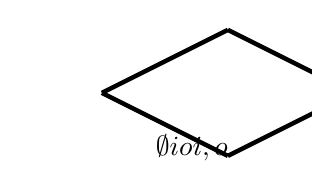
\begin{tikzpicture}[scale=0.8]
            \crd{0}{0}{$\emptyset$}
            \crd[left]{-2}{1}{$\s{i}$}
            \crd[right]{2}{1}{$\s{o}$}
            \crd[right]{0}{2}{$\s{i,o}$}
            \draw [ultra thick] (0,0) -- (2,1);
            \draw [ultra thick] (0,0) -- (-2,1);
            \draw [ultra thick] (-2,1) -- (0,2);
            \draw [ultra thick] (2,1) -- (0,2);
        \end{tikzpicture}
    \end{center}
\end{frame}

\begin{frame}
    \begin{center}
        \begin{tikzpicture}[node distance=15mm]
            \node[r] (moi) {$M_{\s{o},i}$};
            \node[b] (mei) [below right of=moi] {$M_{\e,i}$};
            \node[b] (eei) [below of=mei] {$EN_{\e,i}$};
            \node[b] (eoi) [below left of=eei]{$EN_{\s{o},i}$};
            \draw[->] (moi) -- (mei);
            \draw[->] (mei) -- (eei);
            \draw[->] (eei) -- (eoi);
            \draw[->] (moi) -- (eoi);

            \node[b] (mio) [left of=moi] {$M_{\s{i},o}$};
            \node[r] (meo) [below left of=mio] {$M_{\e,o}$};
            \node[r] (eeo) [below of=meo] {$EN_{\e,o}$};
            \node[o] (eio) [below right of=eeo]{$EN_{\s{i},o}$};
            \draw[->] (mio) -- (meo);
            \draw[->] (meo) -- (eeo);
            \draw[->] (eeo) -- (eio);
            \draw[->] (mio) -- (eio);
        \end{tikzpicture}
        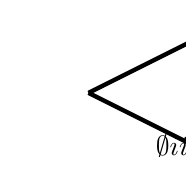
\begin{tikzpicture}[scale=0.8]
            \crd{0}{0}{$\emptyset$}
            \crd[left]{-2}{1}{$\s{i}$}
            \crd[right]{0}{2}{$\s{i,o}$}
            \draw [ultra thick] (0,0) -- (-2,1);
            \draw [ultra thick] (-2,1) -- (0,2);
        \end{tikzpicture}
    \end{center}
\end{frame}

\begin{frame}
    \begin{center}
        \begin{tikzpicture}[node distance=15mm]
            \node[r] (moi) {$M_{\s{o},i}$};
            \node[b] (mei) [below right of=moi] {$M_{\e,i}$};
            \node[b] (eei) [below of=mei] {$EN_{\e,i}$};
            \node[b] (eoi) [below left of=eei]{$EN_{\s{o},i}$};
            \draw[->] (moi) -- (mei);
            \draw[->] (mei) -- (eei);
            \draw[->] (eei) -- (eoi);
            \draw[->] (moi) -- (eoi);

            \node[b] (mio) [left of=moi] {$M_{\s{i},o}$};
            \node[r] (meo) [below left of=mio] {$M_{\e,o}$};
            \node[r] (eeo) [below of=meo] {$EN_{\e,o}$};
            \node[b] (eio) [below right of=eeo]{$EN_{\s{i},o}$};
            \draw[->] (mio) -- (meo);
            \draw[->] (meo) -- (eeo);
            \draw[->] (eeo) -- (eio);
            \draw[->] (mio) -- (eio);
        \end{tikzpicture}
        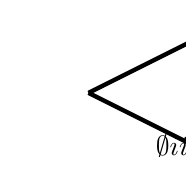
\begin{tikzpicture}[scale=0.8]
            \crd{0}{0}{$\emptyset$}
            \crd[left]{-2}{1}{$\s{i}$}
            \crd[right]{0}{2}{$\s{i,o}$}
            \draw [ultra thick] (0,0) -- (-2,1);
            \draw [ultra thick] (-2,1) -- (0,2);
        \end{tikzpicture}
    \end{center}

    \begin{center}
        \begin{align*}
            \e \vdash i, \s{o} \vdash i, \s{i} \vdash o
        \end{align*}
    \end{center}
\end{frame}
